% Stefan Kottwitz, LaTeX Cookbook, Packt Publishing, 2015
% Chapter 5, Designing Tables
% Adding shape, shading, and transparency
% With automatic row counting
\documentclass{beamer}
\setbeamertemplate{navigation symbols}{}
\setbeamertemplate{background canvas}[vertical shading]%
  [top=blue!1,bottom=blue!40]
\usepackage{booktabs}
\usepackage{tikz}
\usetikzlibrary{calc}
\pgfdeclarelayer{background}
\pgfsetlayers{background,main}
\newcommand{\up}{\textcolor{green}{$\blacktriangle$}}
\newcommand{\down}{\textcolor{red}{$\blacktriangledown$}}
\newcommand{\same}{\textcolor{darkgray}{\textbf{--}}}
\newcommand{\header}[1]{{\Large\bfseries #1\par\medskip}}
\usepackage{array}
\newcounter{rank}
\setcounter{rank}{0}
\newcommand{\steprank}{\stepcounter{rank}\makebox[2em]{\therank}\hspace{\tabcolsep}}
\begin{document}
\begin{frame}
  \centering
  \header{Linux distribution ranking, December 14, 2014}
  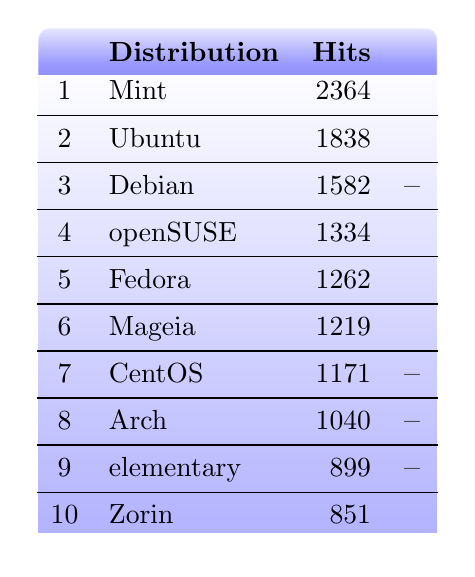
\begin{tikzpicture}
    \node (tbl) {
      \begin{tabular}{@{\steprank}lrcc}
        \multicolumn{1}{l}{\hspace{2em}\textbf{Distribution}} & \textbf{Hits} & \\
        \addlinespace[2pt]
        Mint       & 2364 & \down \\
        \midrule
        Ubuntu     & 1838 & \up \\
        \midrule
        Debian     & 1582 & \same \\
        \midrule
        openSUSE   & 1334 & \up \\
        \midrule
        Fedora     & 1262 & \up \\
        \midrule
        Mageia     & 1219 & \down \\
        \midrule
        CentOS     & 1171 & \same \\
        \midrule
        Arch       & 1040 & \same \\
        \midrule
        elementary &  899 & \same \\
        \midrule
        Zorin      &  851 & \down \\[0.5ex]
      \end{tabular}};
    \begin{pgfonlayer}{background}
      \draw[rounded corners, top color=blue!20,
        bottom color=blue!80!black, middle color=blue!80,
        opacity=0.5, draw=white] ($(tbl.north west)+(0.14,0)$)
        rectangle ($(tbl.north east)-(0.13,0.9)$);
      \draw[top color=blue!1,bottom color=blue!30,draw=white]
        ($(tbl.north east)-(0.13,0.6)$)
        rectangle ($(tbl.south west)+(0.13,0.2)$);
    \end{pgfonlayer}
  \end{tikzpicture}

  \small
  Data by DistroWatch.com, spanning over the last 6 months,
  hits per day.
\end{frame}
\end{document}